% !TEX root = root.tex
% 

\documentclass[letterpaper, 10 pt, conference]{ieeeconf}
%\documentclass[a4paper, 10pt, conference]{ieeeconf}

\input{latex_common/preamble.tex}
\input{latex_common/my_tikz.tex}
\usepackage{subfig}

\newcommand{\ocost}{\phi}

\newcommand{\setEcvx}{\mathcal{E}_{\text{cvx}}}
\newcommand{\setIcvx}{\mathcal{I}_{\text{cvx}}}
\newcommand{\setEncvx}{\mathcal{E}_{\text{ncvx}}}
\newcommand{\setIncvx}{\mathcal{I}_{\text{ncvx}}}

\newcommand{\z}{z}
\newcommand{\nz}{n_{\z}}
\renewcommand{\zb}{\bar{z}}
\newcommand{\vc}{\nu}
\newcommand{\vcc}{\sigma}
\newcommand{\tr}{\eta}
\newcommand{\pmet}{\rho}

% convex/non-convex functions
\newcommand{\fc}{g}
\newcommand{\fni}{h}
\newcommand{\fne}{f}
\newcommand{\fnib}{\bar{\fni}}
\newcommand{\fneb}{\bar{\fne}}

\IEEEoverridecommandlockouts                              % This command is only needed if                                                         % you want to use the \thanks command

\overrideIEEEmargins                                      % Needed to meet printer requirements.

%In case you encounter the following error:
%Error 1010 The PDF file may be corrupt (unable to open PDF file) OR
%Error 1000 An error occurred while parsing a contents stream. Unable to analyze the PDF file.
%This is a known problem with pdfLaTeX conversion filter. The file cannot be opened with acrobat reader
%Please use one of the alternatives below to circumvent this error by uncommenting one or the other
%\pdfobjcompresslevel=0
%\pdfminorversion=4

% See the \addtolength command later in the file to balance the column lengths
% on the last page of the document

% The following packages can be found on http:\\www.ctan.org
%\usepackage{graphics} % for pdf, bitmapped graphics files
%\usepackage{epsfig} % for postscript graphics files
%\usepackage{mathptmx} % assumes new font selection scheme installed
%\usepackage{times} % assumes new font selection scheme installed
%\usepackage{amsmath} % assumes amsmath package installed
%\usepackage{amssymb}  % assumes amsmath package installed

\title{\LARGE \bf Title
}


\author{Taylor P. Reynolds and Mehran Mesbahi% <-this % stops a space
\thanks{*This research has been supported by XXX}% <-this % stops a space
\thanks{The authors are with the W.E. Boeing Department of Aeronautics and Astronautics,
        University of Washington, Seattle, WA, USA.
        {\tt\small \{tpr6,mesbahi\}@uw.edu}}%
}

\begin{document}

\maketitle
\thispagestyle{empty}
\pagestyle{empty}


%%%%%%%%%%%%%%%%%%%%%%%%%%%%%%%%%%%%%%%%%%%%%%%%%%%%%%%%%%%%%%%%%%%%%%%%%%%%%%%%
\begin{abstract}

abstract.

\end{abstract}


%%%%%%%%%%%%%%%%%%%%%%%%%%%%%%%%%%%%%%%%%%%%%%%%%%%%%%%%%%%%%%%%%%%%%%%%%%%%%%%%
\section{INTRODUCTION}\label{sec:intro}

Solving non-convex optimization problems is hard. Unfortunately, non-convex problems are pervasive in both the optimal control literature and practical engineering system design. Examples include most optimal control problems with nonlinear dynamics, problems that have non-convex state constraints, or those with control constraints that cannot ``losslessly convexified''~\cite{Acikmese2011,Blackmore2012b}. Such problems can be found in fields ranging from aerospace~\cite{SzmukReynolds2018,Lee2017,Liu2014} and mechanical truss design~\cite{Beck2010} to power grid technology~\cite{Wei2017} and computer vision~\cite{Jiang2007}. For these non-convex optimal control and parameter optimization problems, sequential convex programming (SCP) is one of several techniques that can be used to find a solution(s). Other techniques may include nonlinear programming~\cite{Gill1981,NocedalWright}, sum of squares optimization~\cite{Parrilo2003,Blekherman2012} and evolutionary algorithms.

Sequential convex programming is a natural approach to solving challenging non-convex optimization problems; convex programming is generally thought of as ``easy'' (from a computational perspective) and the associated theoretical backing is well established~\cite{Rockafellar1970,BoydBook}. All SCP techniques stem from the same idea: solve a sequence of convex approximations to the original non-convex problem, each time using the solution of a previous convex problem to improve the approximation.  The main challenge lies in \textit{how} the convex approximations are formulated, what structure is devised for measuring progress towards an optimal solution and updating the approximations, and how all of this lends itself to theoretical analysis. The purpose of this paper is to demonstrate that certain classes of SCP algorithms are susceptible to what we call the \textit{crawling phenomenon}. The crawling phenomenon is defined as slow progress towards a solution when the algorithm is not close to a solution, and is shown to be a result of the algorithm's construction (hence it is unavoidable for this class of SCP algorithms).

% The idea to solve non-convex optimization problems by iteratively approximating them as convex programs was perhaps first developed using branch and bound techniques~\cite{Falk1969,Soland1971,Horst1984}. Important practical algorithms emerged from these early investigations, e.g., McCormick relaxations~\cite{McCormick1976}, that continue to be developed with increasing computational abilities~\cite{Mitsos2009,Tsoukalas2014,Singer2004}.

Likely the simplest class of SCP methods is that of sequential linear programming (SLP). Algorithms in this class linearize all nonlinear functions about a current reference solution to obtain a linear program. The linear program is solved (with a trust region) to obtain a new reference, and the process repeats~\cite{Byrd2004}. Early developments came from the petroleum industry and were intended to solve large problems~\cite{Palacios-Gomez1982}. From a computational perspective, SLP became attractive early due to the maturity of the simplex algorithm. However, over time solvers for more general classes of convex optimization problems have advanced to the point that restricting oneself to linear programs to save computational resources is unnecessary (except perhaps for extremely large problems).  More general than SLP, difference of convex functions, or d.c.~programming, is a class of SCP methods~\cite{Horst1999}. The convex-concave procedure introduced in~\cite{Yuille2002} decomposes each non-convex inequality constraint into a sum of a convex and concave function. Only the concave part in the sum is linearized, leaving the convex part intact. This procedure remains popular in modern applications, in particular for support vector machines and principal component analysis in the field of machine learning~\cite{Lanckriet2009}. 

Another important class of SCP methods is that of sequential quadratic programming (SQP). The collective works of Han~\cite{Han1977}, Powell~\cite{Powell1978a,Powell1986}, Boggs and Tolle~\cite{Boggs1982,Boggs1989,Boggs1996} and Fukushima~\cite{Fukushima1986} exerted significant influence on the early developments of SQP algorithms, and their impact remains evident today. SQP methods approximate a non-convex program using a quadratic program by forming a quadratic approximation of the original problem's Lagrangian using a reference solution. The quadratic program is solved to obtain a new solution, and the process repeats. SQP methods are arguably the most mature class of SCP methods~\cite{Gill2005,Betts1993}.

The use of quadratic programs requires that all constraints are affine in the solution variable. Many problems of interest are, however, subject to nonlinear constraints (both convex and non-convex). The class of algorithms discussed herein are therefore those that solve a more general convex problem at each iteration (i.e., no a priori restriction to an LP or QP). More importantly, we discuss algorithms that are of trust region type and use slack variables to ensure that each convex approximation is always feasible. This class of SCP methods has been developed largely over the last decade, and represents one of the most active areas of current development~\cite{Mao2016a,Mao2018,Bonalli2019,Bonalli2019b}. The novelty of these works lie in the generality of the technical proofs, which hold for any class of convex constraints after non-convexities have been linearized. This paper uses a prototypical algorithm from this class of SCP methods. Since both SLP and SQP methods are contained within this more general class, our discussion holds for them as well. We show that the crawling phenomenon is a fundamental property of algorithms that use a Lagrangian-like function to measure the accuracy of the convex approximations at each iteration and update the trust region and reference solution accordingly. Essentially, the trust region and solution update rules that form a key component of the theoretical convergence analysis induce the undesirable crawling phenomenon.    

% This paper shows that these types of algorithms can suffer from the crawling phenomenon, whereby the algorithm will make slow progress in regions where the convex approximation does not sufficiently capture the curvature of a non-convex constraint. The crawling phenomenon is shown to be a fundamental limitation that is induced by the update rules that govern how the trust region size is updated between iterations. These update rules are a key component of the theoretical analysis that provides guarantees of convergence to (local) minina of the original non-convex problem as well as convergence rate.

This paper is organized as follows. First, we describe the generic class of SCP algorithms, our nomenclature and notation in~\sref{sec:scp}. In~\sref{sec:crawling} we define the crawling phenomenon and prove that algorithms in this class are susceptible to it. A simple example is provided. Section~\ref{sec:remedies} then provides some discussion on algorithms that may avoid the crawling phenomenon, and~\sref{sec:conclusion} offers concluding remarks.

\section{SEQUENTIAL CONVEX PROGRAMMING}\label{sec:scp}

% \begin{itemize}
% \item provide an overview of SCP methods, similar to a condensed version of CSM.
% \item provide a generalized algorithmic framework for the class of algorithms susceptible to the crawling phenomenon.
% \end{itemize}
% only go so far as to define the linear and nonlinear costs as "original cost" plus "feasibility measure". 

Consider the following optimization problem
\begin{subequations}\label{eq:nlp}
\begin{align}
\min_z &\quad \ocost(\z) &&\null \label{eq:nlp_a} \\
\text{s.t.} &\quad \fc_i(\z) \leq 0, &&\quad i \in \setIcvx \label{eq:nlp_b}\\
&\quad \fni_i (\z) \leq 0, &&\quad i \in \setIncvx \label{eq:nlp_c} \\
&\quad \fne_j(\z) = 0, &&\quad j \in \setEncvx \label{eq:nlp_d}
\end{align}
\end{subequations}
where $\z\in\real^{\nz}$, $\setIcvx = \{1,\ldots,m_i\}$, $\setIncvx=\{m_i+1,\ldots,m_i+n_i\}$ represent the indices of the convex and non-convex inequality constraints and $\setEncvx=\{1,\ldots,n_e\}$ represents the indices of non-convex equality constraints. We shall assume that the cost function $\ocost$ is convex, and that each $\fni_i$ and $\fne_j$ are at least once differentiable almost everywhere. To simplify the notation, we assume that any convex equality constraint is represented by a pair of convex inequality constraints. Problem~\eqref{eq:nlp} is typically refered to as a nonlinear programming problem, but herein we shall refer to it as the original non-convex optimization problem (or simple the original problem). While there exist general purpose solvers that are able to solve the original problem (see, e.g.,~\cite{Gill1981,NocedalWright}), we focus on iterative schemes that are based on convex optimization. 

The barrier to directly applying convex optimization is of course the set of non-convex constraints~\eqref{eq:nlp_c} and~\eqref{eq:nlp_d}. Sequential convex programming methods approximate each of these constraints with a convex function of the solution variable, and iteratively update the approximations based on the solution of the resulting convex program. In this way, the original problem is transformed into a sequence of convex \textit{subproblems}. Each convex approximation is computed using a reference solution, $\zb$, and takes the form
\begin{subequations}\label{eq:cvx_approximation_general}
\begin{align}
\fnib_i(\z,\zb) \leq 0, \quad i\in\setIncvx, \label{eq:cvx_approximation_general_ineq} \\
\fneb_j(\z,\zb) = 0, \quad j\in\setEncvx. \label{eq:cvx_approximation_general_eq}
\end{align}
\end{subequations}
There are several choices for $\fnib_i$: first- or second-order Taylor series approximations, inner convex approximations, or any other convex function that locally approximates the non-convex $h_i$. The $\fneb_j$ on the other hand must be affine functions of $\z$. The approximations $\fnib_i$ and $\fneb_j$ are therefore local; their accuracy decreases as $\|\z-\zb\|$ increases. As a separate issue, consider the possible scenario where $\ocost$ and each $g_i$ are linear functions, and we choose each $\fnib_i$ to be a first-order approximation (i.e., the linearization of $\fni_i$ around $\zb$). In this case, the resulting optimization problem is unbounded below, a phenomenon refered to as \textit{artificial unboundedness}. To address the local nature of the approximations~\eqref{eq:cvx_approximation_general} and to avoid artificial unboundedness, we add a \textit{trust region} constraint of the form
\begin{equation}
\| \z - \zb \|_q \leq \tr,
\label{eq:trust_region}
\end{equation}
where $q=\{1,\,2,\,\infty\}$ and $\tr\in\realpp$ is a positive \textit{trust region radius}. Now we may formulate the following convex approximation to Problem~\eqref{eq:nlp}:
\begin{subequations}\label{eq:cvx_tr}
\begin{align}
\min_z &\quad \ocost(\z) &&\null \label{eq:cvx_tr_a} \\
\text{s.t.} &\quad \fc_i(\z) \leq 0, &&\quad i\in\setIcvx \label{eq:cvx_tr_b} \\
&\quad \fnib_i(\z,\zb) \leq 0, &&\quad i\in\setIncvx \label{eq:cvx_tr_c}\\
&\quad \fneb_j(\z,\zb) = 0, &&\quad j\in\setEncvx \label{eq:cvx_tr_d} \\
&\quad \| \z - \zb \|_q \leq \tr  &&\null \label{eq:cvx_tr_e}
\end{align}
\end{subequations}
Directly solving Problem~\eqref{eq:cvx_tr} has proved to be empirically difficult due to \textit{artificial infeasibility} that stems from two probable causes. First, the approximations~\eqref{eq:cvx_tr_c},~\eqref{eq:cvx_tr_d} and trust region~\eqref{eq:cvx_tr_e} can be incompatible, in the sense that $\mathcal{F}_1 = \{\z\,|\,\eqref{eq:cvx_tr_c},~\eqref{eq:cvx_tr_d}\text{ and }\eqref{eq:cvx_tr_e}\text{ are satisfied}\} = \emptyset$. 
%This may occur when the reference $\zb$ is further than a distance $\tr$ from the set $\{\z\,|\,g_i(\z)\leq0,~i\in\setIcvx\}$ under the $q$-norm. 
Second, the constraints~\eqref{eq:cvx_tr_b},~\eqref{eq:cvx_tr_c} and~\eqref{eq:cvx_tr_d} can be incompatible, in the sense that $\mathcal{F}_2 = \{\z\,|\,\eqref{eq:cvx_tr_b},~\eqref{eq:cvx_tr_c}\text{ and }\eqref{eq:cvx_tr_d}\text{ are satisfied}\}=\emptyset$. Illustrations of these two cases are shown graphically in Figure~\ref{fig:artificial_infeas}. Artificial infeasibility can be avoided by adding so-called \textit{virtual control} to~\eqref{eq:cvx_tr_c} and~\eqref{eq:cvx_tr_d}:
\begin{subequations}\label{eq:virtual_control}
\begin{align}
\fnib_i(\z,\zb) - \vcc_i \leq 0 \\
\fneb_j(\z,\zb) - \vc_j = 0
\end{align}
\end{subequations}
where $\vcc_i > 0$. The vectors $\vcc\in\real^{n_i}$ and $\vc\in\real^{n_e}$ are added as solution variables, and the resulting augmented convex program is%
\begin{figure}
\centering
\subfloat[$\mathcal{F}_1 = \emptyset$.]{% !TEX ROOT = ../root.tex

\begin{tikzpicture}
\tikzmath{
	\hx=1.75; \hy=1.75; \hyy=-1.25;
	\cx=0.70; \cy=0.95;
	\dds=0.035;
	\xintrsct=\cx;
	\xright=0.85;
	\slp=0.5;
}
\tikzstyle{every node}=[font=\footnotesize]

% draw axes
\draw[->] (0,\hyy) -- (0,\hy) node[anchor=east] {$z_2$};
\draw[<->] (-\hx,0) -- (\hx,0) node[anchor=north] {$z_1$};
\foreach \x in {-1,-0.5,0.5,1} \draw[] (\x,-\dds) -- (\x,\dds);
\foreach \y in {-1,-0.5,0.5,1} \draw[] (-\dds,\y) -- (\dds,\y);
% draw trust region
\draw[densely dashed,red,fill=red,fill opacity=0.2] (\cx,\cy) circle (0.4);
\node[anchor=south,red,name=tr] at (\cx+0.3,\cy+0.65) {$\| \z - \zb \|_2 \leq \tr$};
\draw[] (tr.south) to[out=-90,in=90] (\cx,\cy+0.45);
% draw zb
\filldraw[black] (\cx,\cy) circle (1.5pt) node[anchor=south east,yshift=-0.1cm] {$\zb$};
% draw ncvx constraint
\draw[thick,domain=-1:\hy,smooth,variable=\x,blue] plot ({\x},{\slp*\x*\x});
\node[anchor=south,name=ncvx,blue] at (-1,0.5) {$\fne_1(\z)=0$};
% draw cvx linearization
\draw[thick,domain=-0.25:\hy,smooth,variable=\x,dashed,red] plot ({\x},{2*\slp*\xintrsct*\x-\slp*\xintrsct*\xintrsct});
\node[anchor=north,name=cvx,red] at (\cx+0.15,-0.25) {$\fneb_1(\z,\zb)=0$};

\end{tikzpicture}} \hfil
\subfloat[$\mathcal{F}_2 = \emptyset$]{% !TEX ROOT = ../root.tex

\begin{tikzpicture}
\tikzmath{
	\hx=1.75; \hy=1.75; \hyy=-1.25;
	\cx=0.40; \cy=0.5;
	\dds=0.035;
	\xintrsct=\cx;
	\xright=0.85;
	\slp=0.5;
	\bx=1.5; \mMm=-0.15; \bBb=1;
	\cXx=0.2; \dXx=0.06;
}
\tikzstyle{every node}=[font=\footnotesize]

% draw axes
\draw[->] (0,\hyy) -- (0,\hy) node[anchor=east] {$z_2$};
\draw[<->] (-\hx,0) -- (\hx,0) node[anchor=north] {$z_1$};
\foreach \x in {-1,-0.5,0.5,1} \draw[] (\x,-\dds) -- (\x,\dds);
\foreach \y in {-1,-0.5,0.5,1} \draw[] (-\dds,\y) -- (\dds,\y);
% draw trust region
\draw[densely dashed,red,fill=red,fill opacity=0.2] (\cx,\cy) circle (0.5);
% \node[anchor=south,red,name=tr] at (\cx+0.3,\cy+0.65) {$\| \z - \zb \|_2 \leq \tr$};
% \draw[] (tr.south) to[out=-90,in=90] (\cx,\cy+0.45);
% draw zb
\filldraw[black] (\cx,\cy) circle (1.5pt) node[anchor=south east,yshift=-0.1cm] {$\zb$};
% draw ncvx constraint
\draw[thick,domain=-1:\hy,smooth,variable=\x,blue] plot ({\x},{\slp*\x*\x});
\node[anchor=south,name=ncvx,blue] at (-1,0.5) {$\fne_1(\z)=0$};
% draw cvx linearization
\draw[thick,domain=-0.5:\hy,smooth,variable=\x,dashed,red] plot ({\x},{2*\slp*\xintrsct*\x-\slp*\xintrsct*\xintrsct});
\node[anchor=north,name=cvx,red] at (-0.5,-0.25) {$\fneb_1(\z,\zb)=0$};
% draw inequality g1
\draw[thick,domain=-0.5:\hy,smooth,variable=\x,darkgreen] plot ({\x},{\mMm*\x+\bBb});
\draw[darkgreen,->] (\cXx-0.0707,\mMm*\cXx+\bBb+0.0707) -- ++(\dXx,-\dXx/\mMm);
\node[anchor=south,darkgreen] at (-1,1.1) {$\fc_1(\z) \leq 0$};
% draw inequality g2
\draw[thick,darkgreen] (\bx,-1) -- (\bx,1.5);
\draw[darkgreen,->] (\bx-0.1,-0.8) -- ++(-0.4,0); 
\node[anchor=north,darkgreen] at (\bx,-1) {$\fc_2(\z)\leq0$};


\end{tikzpicture}}
\caption{A depiction of the two causes of artificial infeasibility.}
\label{fig:artificial_infeas}
\end{figure}
\begin{subequations}\label{eq:cvx_apprx}
\begin{align}
\min_{\z,\vcc,\vc} &\quad \ocost(\z) + \lambda P(\vcc,\vc) &&\null \label{eq:cvx_apprx_a} \\
\text{s.t.} &\quad \fc_i(\z) \leq 0, &&\quad i\in\setIcvx \label{eq:cvx_apprx_b} \\
&\quad \fnib_i(\z,\zb) - \vcc_i \leq 0, &&\quad i\in\setIncvx \label{eq:cvx_apprx_c}\\
&\quad \fneb_j(\z,\zb) - \vc_j = 0, &&\quad j\in\setEncvx \label{eq:cvx_apprx_d} \\
&\quad \|\z-\zb\|_q \leq \tr &&\null  \label{eq:cvx_apprx_e}
\end{align}
\end{subequations}
where $P : \real^{n_e}\times\real^{n_i} \rightarrow \realpp$ is a positive-definite penalty function and $\lambda>0$ is a user-selected weight. Typically $\lambda \gg 1$ to limit the use of virtual control only to cases when it is required to avoid artificial infeasibility.

We shall refer to a solution to Problem~\eqref{eq:cvx_apprx} as an \textit{iterate}, and denote it by $(\z^*,\vcc^*,\vc^*)$. Sequential convex programming algorithms iteratively solve Problem~\eqref{eq:cvx_apprx} and use the resulting iterate to update $\zb$. Moreover, the iterate $(\z^*,\vcc^*,\vc^*)$ is used to update the value of $\tr$, based on some assessment of the accuracy of the approximation in~\eqref{eq:cvx_approximation_general}. The resulting sequence of solutions $\zb$ approaches a locally optimal solution of~\eqref{eq:nlp} under certain conditions and problem assumptions. There have been numerous papers that study the convergence properties of these algorithms, offering conditions/assumptions under which convergence is guaranteed to various definitions of minima~\cite{Mao2016a,Mao2018,Bonalli2019,Bonalli2019b}. This paper does not discuss \textit{whether} convergence is achieved or at what rate, but instead looks at an implicit property of algorithms that use the accuracy of the convex approximation~\eqref{eq:cvx_apprx} to update $\zb$ and $\tr$.

\subsection{Trust Region Updates}\label{subsec:tr_updates}

Most sequential convex programming methods dynamically update the value of $\tr$ at each iteration according to a set of specified rules. These rules are designed to facilitate formal convergence proofs, and make use of a performance metric that is a function of $(\z^*,\vcc^*,\vc^*)$ to do so. The performance metric provides key feedback to the iterative process and guides convergence. To introduce a few common performance metrics, we first define the following functions
\begin{subequations}\label{eq:scp_costs}
\begin{align}
J(\z) &= \ocost(\z) + \lambda P\big( \fni(\z),\,\fne(\z) \big) \label{eq:scp_costs_nl}\\
L(\z) &= \ocost(\z) + \lambda P\big( \fnib(\z,\zb),\,\fneb(\z,\zb) \big) \label{eq:scp_costs_l}
\end{align}
\end{subequations}
where $\fni(\z) \in \real^{n_i}$ and $\fne(\z)\in\real^{n_e}$ are the concatenations of the non-convex constraints from the original problem~\eqref{eq:nlp_c}, and similarly for $\fnib(\z,\zb)$ and $\fneb(\z,\zb)$. The cost functions in~\eqref{eq:scp_costs} can be thought of as approximations of the Lagrangians of the original problem, for~\eqref{eq:scp_costs_nl}, and the convex subproblem for~\eqref{eq:scp_costs_l}. 
%
 % measuring the optimality (via $\ocost$) and the feasibility (via $P(\cdot,\cdot)$) of a candidate solution. The measure of feasibility is weighted by $\lambda$. The function~\eqref{eq:scp_costs_nl} measures this weighted cost with respect to the original non-convex problem~\eqref{eq:nlp}, while the function~\eqref{eq:scp_costs_l} measures the same weighted cost with respect to the approximated convex problem~\eqref{eq:cvx_apprx}. 
%
We now introduce two commonly used performance metrics. The first is simply the \textit{relative error}
\begin{equation}
\pmet = \frac{J(\z^*) - L(\z^*)}{L(\z^*)},
\label{eq:pmet_rel_error}
\end{equation}
which measures the normalized difference in the approximated Lagrangians. The ideal value of the relative error is zero. Another performance metric is the \textit{relative decrement} defined as
\begin{equation}
\pmet = \frac{J(\zb) - J(\z^*)}{J(\zb) - L(\z^*)},
\label{eq:pmet_rel_decrement}
\end{equation}
which measures how well the convex approximation predicts the change in the original problem's approximated Lagrangian. The ideal value of the relative decrement is one. Once chosen\footnote{We stress that the choice of performance metric is not arbitrary, but is tied to the use of a specific algorithm. The two possibilities presented here are abstract representations of performance metrics used by algorithms in the literature.}, the scalar-valued performance metric $\pmet$ is used to grow, shrink, or maintain the size of the trust region radius. Crucially, it is also used to reject a solution $\z^*$ in certain cases. If $\pmet$ indicates poor prediction in behavior, the same convex approximation is kept but the trust region is shrunk, and the convex subproblem is re-solved. 

To decide which case we are in for a given iteration (accept/reject, shrink/keep/grow), the user defines three real numbers $\pmet_0,\,\pmet_1,\,\pmet_2\in(0,1)$ that split the real number line into four segments. The value of $\pmet$ places each iterate into one of these four segments, and the trust region and reference solution are updated according to the rules in Figure~\ref{fig:scp_updates}. The constants $\alpha,\beta >1$ are user-selected the shrink and growth rates, respectively. 

\begin{figure*}
\centering
% !TEX ROOT = ../root.tex

\begin{tikzpicture}
\tikzmath{
	\cx=0; \cy=0; \wdt=2.5; \hgt=2;
	\dx=0.25; \dxx=0.7;
	\cxx=\cx+\wdt+\dx; 
	\cxxx=\cxx+\wdt+\dx;
	\civ=\cxxx+\wdt+\dx;
	\Rly=\cy-0.5*\hgt-2*\dx;
	\cyy=\Rly-2.5*\dx;
	\cyyy=\Rly+2.5*\dx;
}
\tikzstyle{every node}=[font=\small]

% NUMBER LINE
\begin{scope}[shift={(0,\Rly)}]
% rho_0
\draw[thick,dashed] (\cx+0.5*\wdt+0.5*\dx,6*\dx) -- (\cx+0.5*\wdt+0.5*\dx,-6*\dx) node[anchor=south,pos=0] {$\rho_0$};
% rho_1
\draw[thick,dashed] (\cxx+0.5*\wdt+0.5*\dx,6*\dx) -- (\cxx+0.5*\wdt+0.5*\dx,-6*\dx) node[anchor=south,pos=0] {$\rho_1$};
% rho_2
\draw[thick,dashed] (\cxxx+0.5*\wdt+0.5*\dx,6*\dx) -- (\cxxx+0.5*\wdt+0.5*\dx,-6*\dx) node[anchor=south,pos=0] {$\rho_2$};
% reals
\draw[ultra thick,<->] (\cx-0.5*\wdt-2*\dx,0) -- (\civ+0.5*\wdt+2*\dx,0) node[anchor=west] {\Large $\real$};
\end{scope}

%% TOP TEXT
\node[anchor=south] at (\cx,\cy-\dx) {$\pmet < \pmet_0$};
\node[anchor=south] at (\cxx,\cy-\dx) {$\pmet \in [\pmet_0,\pmet_1)$};
\node[anchor=south] at (\cxxx,\cy-\dx) {$\pmet\in[\pmet_1,\pmet_2)$};
\node[anchor=south] at (\civ,\cy-\dx) {$\pmet \geq \pmet_2$};

%% TOP BOXES
% Case 1
\pane{\cx}{\cyy}{0}{\wdt}{0.5*\hgt}{0.2}{draw,color=red!50!white,fill=red!10!white}
\node[] at (\cx,\cyy) {\begin{tabular}{l}
$\tr \leftarrow \tr / \alpha $ \\
$\zb \leftarrow \zb$ 
\end{tabular}};

% Case 2
\pane{\cxx}{\cyy}{0}{\wdt}{0.5*\hgt}{0.2}{draw,color=yellow!70!black,fill=yellow!10!white}
\node[] at (\cxx,\cyy) {\begin{tabular}{l}
$\tr \leftarrow \tr / \alpha$ \\
$\zb \leftarrow \z^*$ 
\end{tabular}};

% Case 3
\pane{\cxxx}{\cyy}{0}{\wdt}{0.5*\hgt}{0.2}{draw,color=green!50!white!80!black,fill=green!10!white}
\node[] at (\cxxx,\cyy) {\begin{tabular}{l} 
$\tr \leftarrow \tr$ \\
$\zb \leftarrow \z^*$ 
\end{tabular}};

% Case 4
\pane{\civ}{\cyy}{0}{\wdt}{0.5*\hgt}{0.2}{draw,color=green!50!white!80!black,fill=green!10!white}
\node[] at (\civ,\cyy) {\begin{tabular}{l}
$\tr \leftarrow \beta \tr$ \\
$\zb \leftarrow \z^*$
\end{tabular}};

%% BOTTOM BOXES
% Case 1
\pane{\cx}{\cyyy}{0}{\wdt}{0.5*\hgt}{0.2}{draw,color=green!50!white!80!black,fill=green!10!white}
\node[] at (\cx,\cyyy) {\begin{tabular}{l}
$\tr \leftarrow \beta \tr $ \\
$\zb \leftarrow \z^*$ 
\end{tabular}};

% Case 2
\pane{\cxx}{\cyyy}{0}{\wdt}{0.5*\hgt}{0.2}{draw,color=green!50!white!80!black,fill=green!10!white}
\node[] at (\cxx,\cyyy) {\begin{tabular}{l}
$\tr \leftarrow  \tr$ \\
$\zb \leftarrow \z^*$ 
\end{tabular}};

% Case 3
\pane{\cxxx}{\cyyy}{0}{\wdt}{0.5*\hgt}{0.2}{draw,color=yellow!70!black,fill=yellow!10!white}
\node[] at (\cxxx,\cyyy) {\begin{tabular}{l}
$\tr \leftarrow \tr / \alpha$ \\
$\zb \leftarrow \z^*$ 
\end{tabular}};

% Case 4
\pane{\civ}{\cyyy}{0}{\wdt}{0.5*\hgt}{0.2}{draw,color=red!50!white,fill=red!10!white}
\node[] at (\civ,\cyyy) {\begin{tabular}{l}
$\tr \leftarrow \tr / \alpha$ \\
$\zb \leftarrow \zb$
\end{tabular}};

%% LEFT TEXT
\node[text width=2cm, anchor=east, align=right] at (\cx-0.5*\wdt-2*\dx,\cyy) {\textit{Rel.~decrement}};
\node[text width=2cm, anchor=east, align=right] at (\cx-0.5*\wdt-2*\dx,\cyyy) {\textit{Rel.~error}};

\end{tikzpicture}
\caption{Update rules for two different performance metrics of a general sequential convex programming algorithm.}
\label{fig:scp_updates}
\end{figure*}

We now make a brief technical comment before proceeding. First, the denominators in~\eqref{eq:pmet_rel_error} and~\eqref{eq:pmet_rel_decrement} must be verified to be non-zero before computing the value of $\pmet$. In the case of~\eqref{eq:pmet_rel_error}, a necessary and sufficient condition to avoid this is $\ocost(\z)\ne0$ for all feasible $\z$. In the case of~\eqref{eq:pmet_rel_decrement}, a zero denominator actually implies that the iterations can be terminated, since $L(\z^*) \leq L(\zb) = J(\zb)$ (note that this implies the denominator is always nonnegative). If $J(\zb)-L(\z^*)=0$, then the optimal solution found by solving~\eqref{eq:cvx_apprx} is exactly the reference solution, and the iterations may be stopped. Therefore for either performance metric, divide-by-zero conditions can be avoided.   

\section{THE CRAWLING PHENOMENON}\label{sec:crawling}

% A dynamically sized trust region allows an SCP algorithm to take larger steps in regions where the convex approximation is the most accurate. The problem is that the size of the regions where the approximation is accurate can be small, and this is driven by the form of the original non-convex equality constraints~\eqref{eq:nlp_d}. Nonlinear equality constraints force an SCP algorithm that uses the update rules of Figure~\ref{fig:scp_updates} to take small steps, even if we know, for example, that the reference is feasible. 

An algorithm exhibits the \textit{crawling phenomenon} when it is \textit{forced} to take incrementally smaller steps, as measured by $\|\z^*-\zb\|_q$, for iterates $\z^*$ that are not close to a stationary point of the original problem. This section explores the relationship between the crawling phenomenon and the class of SCP algorithms defined in~\sref{sec:scp} that use either~\eqref{eq:pmet_rel_error} or~\eqref{eq:pmet_rel_decrement}.

\subsection{Relative Error}\label{subsec:creep_rel_err}

We first discuss algorithms that use the relative error~\eqref{eq:pmet_rel_error} as the performance metric. From Figure~\ref{fig:scp_updates}, the algorithm will reject the current step if $\pmet\geq\pmet_2$, where $\pmet_2<1$ is a user-defined value. It is enough for the current discussion to assume that $\pmet_2=1$, so that subsequent results are sufficient for any chosen value of $\pmet_2$ during implementation. In order that an iterate be accepted, we must then have
\begin{equation}
\frac{J(\z^*) - L(\z^*)}{L(\z^*)} < 1 \quad \Rightarrow \quad  J(\z^*) < 2 L(\z^*).
\label{eq:rel_err_accept}
\end{equation} 
Using~\eqref{eq:scp_costs} this can be rewritten as
\begin{equation}
P\big( \fni(\z^*),\fne(\z^*) \big) < \frac{\phi(\z^*)}{\lambda} + 2 P\big( \fnib(\z^*,\zb),\fneb(\z^*,\zb) \big).
\label{eq:rel_err_accept_2}
\end{equation}
What~\eqref{eq:rel_err_accept_2} says is that in order for a step to be accepted, the degree to which the iterate $\z^*$ is infeasible for the original non-convex problem must be bounded by the right hand side. If inequality~\eqref{eq:rel_err_accept_2} is violated, we find ourselves in the top-right case in Figure~\ref{fig:scp_updates}: $\z^*$ is rejected, the trust region is shrunk and the subproblem is resolved. The inequality~\eqref{eq:rel_err_accept_2} can also be interpreted as saying that the infeasibility of all accepted iterates with respect to the original non-convex problem is bounded from above by the sum of the (weighted) original cost and twice the amount of infeasibility in the convex approximation. 

Suppose now that the reference $\zb$ is feasible for the original problem, in the sense that $P\big(\fni(\zb),\fne(\zb)\big)=0$. This implies that $\zb$ is a feasible point for the convex subproblem~\eqref{eq:cvx_tr} as well (the convex approximation with no virtual control). Thus the optimal solution of the convex subproblem~\eqref{eq:cvx_apprx} will not use any virtual control provided that $\lambda$ is large enough\footnote{There exists a non-empty feasible set that uses no virtual control, solutions that are not in this set necessarily increase the cost for large values of $\lambda$.}. The solution $\z^*$ will therefore satisfy $\fnib(\z^*,\zb)\leq0$ and $\fneb(\z^*,\zb)=0$. If either $\fnib(\cdot,\zb)$ (resp.~$\fneb(\cdot,\zb)$) does not adequately capture the behavior of $\fni(\cdot)$ (resp.~$\fne(\cdot)$), then inequality~\eqref{eq:rel_err_accept_2} will be violated. This implies that for a given set of non-convex functions $\fni(\cdot)$ and $\fne(\cdot)$, for every feasible $\zb$ there is an \textit{effective maximum trust region size} that is implicitly defined by the method used to ``convexify'' the original problem and the value of the original cost (weighted by $1/\lambda$). This can happen quite easily when, for example, $\fne(\z)$ has a large Lipschitz constant in the set defined by the trust region, and the affine approximation $\fneb_i(\cdot,\zb)$ cannot sufficient capture its curvature. Figure~\ref{fig:effective_tr} provides a depiction of this scenario, while the following Lemma formalizes the statement.

\begin{lemma}\label{lemma:rel_err_effective_tr}
Given a nonlinear programming problem of the form~\eqref{eq:nlp}, and a reference solution $\zb$ that is feasible for~\eqref{eq:nlp}, the solution to the convex approximation~\eqref{eq:cvx_apprx} will be rejected by any algorithm that uses~\eqref{eq:pmet_rel_error} in conjunction with the update rules in Figure~\ref{fig:scp_updates} until
\begin{equation}
\left\{\z\,|\,\|\z-\zb\|_q \leq \eta \right\} \subset \left\{\z\,|\,P\big(\fni(\z),\fne(\z)\big) < \tfrac{\ocost(\z)}{\lambda} \right\},
\label{eq:rel_err_effective_tr}
\end{equation}
for any $q\in\{1,2,\infty\}$. %The left hand side of~\eqref{eq:rel_err_effective_tr} defines an effective maximum trust region size for each feasible reference $\zb$.
\end{lemma}

% Lemma~\ref{lemma:rel_err_effective_tr} can be extended to the case where $\zb$ is not feasible in a straightforward manner. We have presented it as such because for infeasible $\zb$, the right hand side of~\eqref{eq:rel_err_accept_2} implies a larger effective maximum trust region that does not typically hinder progress. The limiting case that serves as the root cause of the crawling phenomenon is when $\zb$ is feasible for the original problem.

\subsection{Relative Decrement}\label{subsec:crepp_rel_dec}

% Algorithms that use the relative decrement as the performance metric exhibit the crawling phenomenon only when the reference is feasible (or nearly so) for the original non-convex problem. In this case, we have $P\big(\fni(\zb),\,\fne(\zb)\big)=0$. 
When using the relative decrement as the performance metric, recall that an iterate may be rejected when $\pmet<\pmet_0$ for some $\pmet_0>0$. Similar to the relative error case, we may assume that $\pmet_0=0$ so that the following results are sufficient for any chosen value. If $\pmet_0=0$, then according to the rules in Figure~\ref{fig:scp_updates} an iterate will only accepted if the \textit{numerator} of~\eqref{eq:pmet_rel_decrement} is strictly positive (recall that the denominator is always nonnegative). Hence for an accepted step we have $0 < J(\zb) - J(\z^*)$ and
\begin{equation}
 P\big( \fni(\z^*),\fne(\z^*) \big) < \frac{\ocost(\zb) - \ocost(\z^*)}{\lambda} + P\big(\fnib(\z^*,\zb),\fneb(\z^*,\zb)\big) \label{eq:rel_dec_bound_c}
\end{equation}
which says that the amount by which the iterate $\z^*$ is infeasible for the original problem is bounded by the (weighted) reduction in original cost plus the amount of virtual control. If inequality~\eqref{eq:rel_dec_bound_c} is violated, we find ourselves in the bottom-left case in Figure~\ref{fig:scp_updates}: $\z^*$ is rejected, the trust region shrunk, and the subproblem is resolved. 

\begin{remark}
The inequality~\eqref{eq:rel_dec_bound_c} also illuminates the fact that if the reference $\zb$ is feasible for the original non-convex problem, then an accepted iterate must (strictly) decrease the original cost. This is due to the fact that $\lambda>0$ and $P(\cdot,\cdot)$ is positive definite. A similar fact was noted for SLP in~\cite{Palacios-Gomez1982}, and hence this property holds for the more general class of algorithms discussed here.
\end{remark}
%
% \begin{remark}
% Even in the reference $\zb$ is not exactly feasible, inequality~\eqref{eq:rel_dec_bound_c} still leads to an upper bound on the infeasibility of the accepted solution. Indeed, if $P\big(\fni(\zb),\fne(\zb)\big)=\epsilon$, then the bound is simply the right hand side of~\eqref{eq:rel_dec_bound_c} plus $\epsilon$. For small $\epsilon$, this both guards against the solution deviating too far from feasibility once it is obtained, while also inducing the crawling phenomenon when $\zb$ is nearly feasible. 
% \end{remark}

Suppose now that $\zb$ is feasible for the original problem, then similar to the case for the relative error, we know that the solution $\z^*$ will satisfy $\fnib(\z^*,\zb)\leq 0$ and $\fneb(\z^*,\zb)=0$. We are thus led to the existence of a maximum effective trust region size that is implicitly defined by the method used to convexify the original problem and the largest possible reduction in the original cost in the feasible set of the convex approximation with no virtual control~\eqref{eq:cvx_tr} (since we know that $\z^*$ will be feasible for this problem). 

\begin{lemma}
Given a nonlinear programming problem of the form~\eqref{eq:nlp} and a reference solution $\zb$ that is feasible for~\eqref{eq:nlp}, the solution to the convex approximation~\eqref{eq:cvx_apprx} will be rejected by any algorithm that uses~\eqref{eq:pmet_rel_decrement} in conjunction with the update rules in Figure~\ref{fig:scp_updates} until
\begin{equation}
\left\{ \z\,|\,\|\z-\zb\|_q \leq \eta \right\} \subseteq \left\{ \z\,|\, P\big(\fni(\z),\fne(\z)\big) < \tfrac{\ocost(\zb)-\ocost(\z)}{\lambda} \right\},
\end{equation}
for any $q\in\{1,2,\infty\}$. 
\end{lemma}

% we know that actually $\zb$ is a feasible point for Problem~\eqref{eq:cvx_tr} as well (the convex approximation with no virtual control). Thus the optimal solution of Problem~\eqref{eq:cvx_apprx} will not use any virtual control provided that $\lambda$ is large enough\footnote{There exists a non-empty feasible set that uses no virtual control, solutions that are not in this set necessarily increase the cost for large values of $\lambda$.}. The solution $\z^*$ will therefore satisfy $\fnib(\z^*,\zb)\leq 0$ and $\fneb(\z^*,\zb)=0$. If either $\fnib(\cdot,\zb)$ (resp.~$\fneb(\cdot,\zb)$) does not adequately capture the behavior of $\fni(\cdot)$ (resp.~$\fne(\cdot)$), then inequality~\eqref{eq:rel_dec_bound_c} is likely to be violated. This implies that for a given set of non-convex functions $\fni(\cdot)$ and $\fne(\cdot)$, for every feasible $\zb$ there is a \textit{maximum trust region size} that is implicitly defined by the method used to ``convexify'' the original problem and the largest achievable reduction in cost (weighted by $1/\lambda$). For $\lambda\gg1$ the maximum trust region size such that~\eqref{eq:rel_dec_bound_c} is satisfied can be small, causing the algorithm to take small incremental steps that are each nearly feasible for the original non-convex problem. This is depicted in Figure~\ref{fig:effective_tr} and is the root cause of the crawling phenomenon.

We may summarize the discussion of the crawling phenomenon for both performance metrices as follows.
\begin{theorem}
Given a nonlinear programming problem of the form~\eqref{eq:nlp}, parameters $\pmet_0,\pmet_1,\pmet_2\in(0,1)$, $\alpha,\beta,\lambda>1$, $q\in\{1,2,\infty\}$, a positive definite function $P:\real^{n_e}\times\real^{n_i}\rightarrow\realpp$, and an initial reference and trust region size $\{\zb,\tr\}$, any algorithm that iteratively solves the convex approximation~\eqref{eq:cvx_apprx} and updates the reference and trust region size using either~\eqref{eq:pmet_rel_error} or~\eqref{eq:pmet_rel_decrement} in conjunction with the rules in Figure~\ref{fig:scp_updates} is subject to the crawling phenomenon.
\end{theorem}

\begin{figure}
\centering
% !TEX ROOT = ../root.tex

\begin{tikzpicture}[scale=1]
\tikzmath{
	\hx=3; \hy=3; \hyy=-1;
	\slp=0.5; \b=0.5;
	\cx=1; \cy=\b+\slp*\cx*\cx;
	\trrad=0.9; \grrad=0.4*\trrad;
	\xj=0.36;
	\yj=\b+2*\slp*\cx*\xj-\slp*\cx*\cx;
	\xjj=\cx-0.05; \yjj=2*\cx*\xjj-\cx*\cx;
	\xjjj=\cx+0.05; \yjjj=2*\cx*\xjjj-\cx*\cx;
}

% draw axes
\draw[thick,->] (0,\hyy) -- (0,\hy) node[anchor=east] {$z_2$};
\draw[thick,<->] (-\hx,0) -- (\hx,0) node[anchor=north,pos=0.97] {$z_1$};
\foreach \x in {-1,-0.75,...,2.75} \draw[dashed,gray,opacity=0.4] (-\hx,\x) -- (\hx,\x); 
\node[anchor=south west,gray] at (-\hx-0.1,2.4) {\footnotesize cost lines};

% blue curve
\draw[thick,domain=-1:2.25,smooth,variable=\x,blue] plot ({\x},{\b+\slp*\x*\x});
\node[blue,align=left,anchor=south east,name=fz] at (-1,0.9) {$\fne(\z) = 0$};

% red curve
\draw[thick,domain=-0.5:2.25,smooth,variable=\x,red] plot ({\x},{\b+2*\slp*\cx*\x-\slp*\cx*\cx});
\node[red,align=center,anchor=south east,name=fz_lin] at (-0.5,-1) {$\fneb(\z,\zb) = 0$};

% trust region
\draw[densely dotted,thick,red,fill=red,fill opacity=0.2,text opacity=1] (\cx,\cy) circle (\trrad) node[anchor=south,yshift=0.9cm,xshift=-0.73cm,text width=3cm,align=center] {\footnotesize current trust region};
\filldraw[black] (\cx,\cy) circle (2pt) node[anchor=south east,yshift=-0.1cm] {$\bar{z}$};

% cyan dot and cost decrease
% \filldraw[cyan] (\xj,\yj) square (2pt);
\node[rectangle,fill=cyan,shift={(\xj,\yj)},scale=0.75] {};% square (2pt);
% \draw[thick,|-|] (\hx-0.8,\cy) -- (\hx-0.8,\yj) node[anchor=west,pos=0.5,text width=2.5cm] {\footnotesize max cost decrease};

% green circle + text
\draw[densely dotted,thick,darkgreen,fill=darkgreen,fill opacity=0.2,text opacity=1] (\cx,\cy) circle (\grrad) node[anchor=south,name=gcirc,yshift=-{\grrad}cm] {};
\node[darkgreen,text width=2.5cm,align=center,anchor=north,name=gtext] at (\cx+0.25,-0.35) {\footnotesize max trust region due to~\eqref{eq:rel_err_accept_2} or~\eqref{eq:rel_dec_bound_c}};
\draw[darkgreen,->] (gtext.north) to[out=90,in=-90] (gcirc.south);

\end{tikzpicture}

\caption{The effective maximum trust region size that induces the crawling phenomenon. The cyan square solution is rejected since it is too far from the curve $\fne(\z)=0$ and the inequality~\eqref{eq:rel_err_accept_2} or~\eqref{eq:rel_dec_bound_c} is violated. The green circle is the largest trust region such that the inequality~\eqref{eq:rel_err_accept_2} or~\eqref{eq:rel_dec_bound_c} is satisfied at the proposed solution.}
\label{fig:effective_tr}
\end{figure}

\subsection{A Simple Example}\label{subsec:toy_example}

This section provides a simple example that exhibits the crawling phenomenon. Consider the following optimization problem in the variable $\z=(z_1,z_2)\in\real^2$
\begin{subequations}\label{eq:toy_prob}
\begin{align}
\min_{\z} &\quad z_1+z_2 \label{eq:toy_prob_a}\\
\text{s.t.} &\quad \fc_1(\z) = -z_2 - \tfrac{4}{3} z_1 - \tfrac{2}{3} \leq 0 \label{eq:toy_prob_b}\\
&\quad \fc_2(\z) = \z - 2 \leq 0 \label{eq:toy_prob_c}\\
&\quad \fc_3(\z) = -\z - 2 \leq 0 \label{eq:toy_prob_d}\\
&\quad \fne(\z) = z_2 - z_1^4 - 2z_1^3 + 1.2z_1^2 + 2z_1 = 0 \label{eq:toy_prob_e}
\end{align}
\end{subequations}
This problem is non-convex due to the quartic constraint~\eqref{eq:toy_prob_e}. Following the procedure outlined in~\sref{sec:scp}, we can convexify Problem~\eqref{eq:toy_prob} for use in an SCP algorithm by introducing the reference $\zb\in\real^2$ and virtual control $\vc\in\real$:
\begin{subequations}\label{eq:toy_prob_cvx}
\begin{align}
\min_{\z,\vc} &\quad z_1+z_2 + \lambda P(\vc) \\
\text{s.t.} &\quad \fc_1(\z) \leq 0,~\fc_2(\z)\leq0,~\fc_3(\z)\leq0 \\
&\quad \fne(\zb) + \jacobev{\fne}{z}{\zb}\tran\left( \z - \zb \right) + \vc = 0 \\
&\quad \twonorm{\z - \zb} \leq \eta
\end{align}
\end{subequations}
The data used for this particular example are an initial trust region of $\eta=0.1$, an initial reference of $\zb=(1.5,1.5)$, a penalty function $P(\vc) = | \vc |$ and $\lambda=400$. The values used to update the trust region size are $\big(\pmet_0,\pmet_1,\pmet_2\big)=(0,0.1,0.9)$ and $\big(\pmet_0,\pmet_1,\pmet_2)=(0.1,0.9,1.0)$ for the relative decrement and relative error respectively, and $\alpha=1.5,\,\beta=2.0$. Figure~\ref{fig:toy_prob_soln} shows the resulting sequence of iterates for both performance metrics, as well as the value of $\pmet$ in each case as a function of the iteration number. Figures~\ref{fig:toy_prob_soln_a} and~\ref{fig:toy_prob_soln_b} demonstrate the crawling phenomenon; progress towards a solution slows down considerably once the curvature of the equality constraint increases towards the bottom. Notice that fairly rapid progress is made initially in both cases when the non-convex function is locally quite linear. In both cases, Figure~\ref{fig:toy_prob_soln_c} reveals a cycle that is reached whereby the approximation accuracy slowly worsens until the trust region is shrunk (the sharp changes in $\pmet$ indicate when the trust region was shrunk). This can be thought of as the nonlinear equality function bending away from the affine approximation, reducing the size of the effective trust region noted in Figure~\ref{fig:effective_tr}. 

\begin{figure*}
\centering
\subfloat[Relative decrement solution, $120$ iterations.\label{fig:toy_prob_soln_a}]{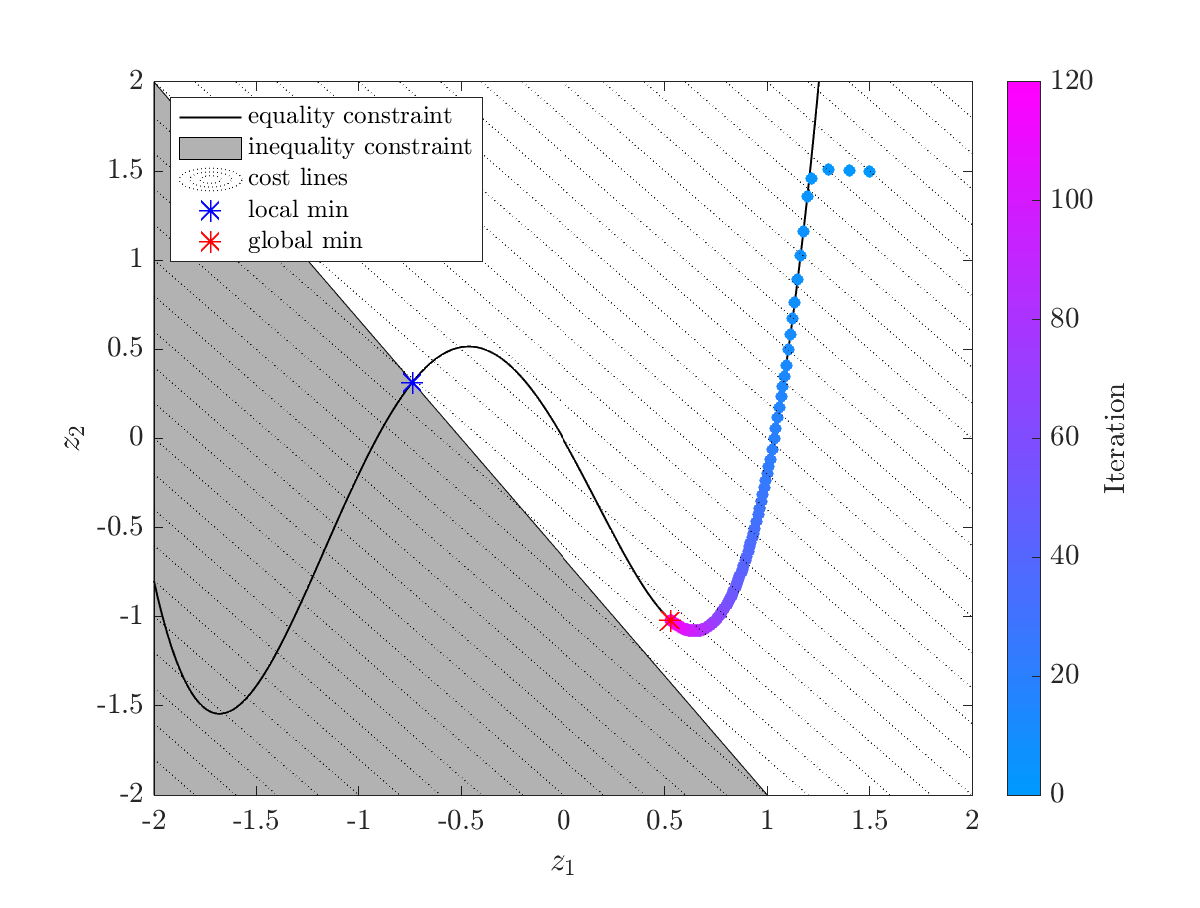
\includegraphics[width=0.33\textwidth]{figs/acc_toy_problem_cvrg_w2}} 
\subfloat[Relative error solution, $65$ iterations.\label{fig:toy_prob_soln_b}]{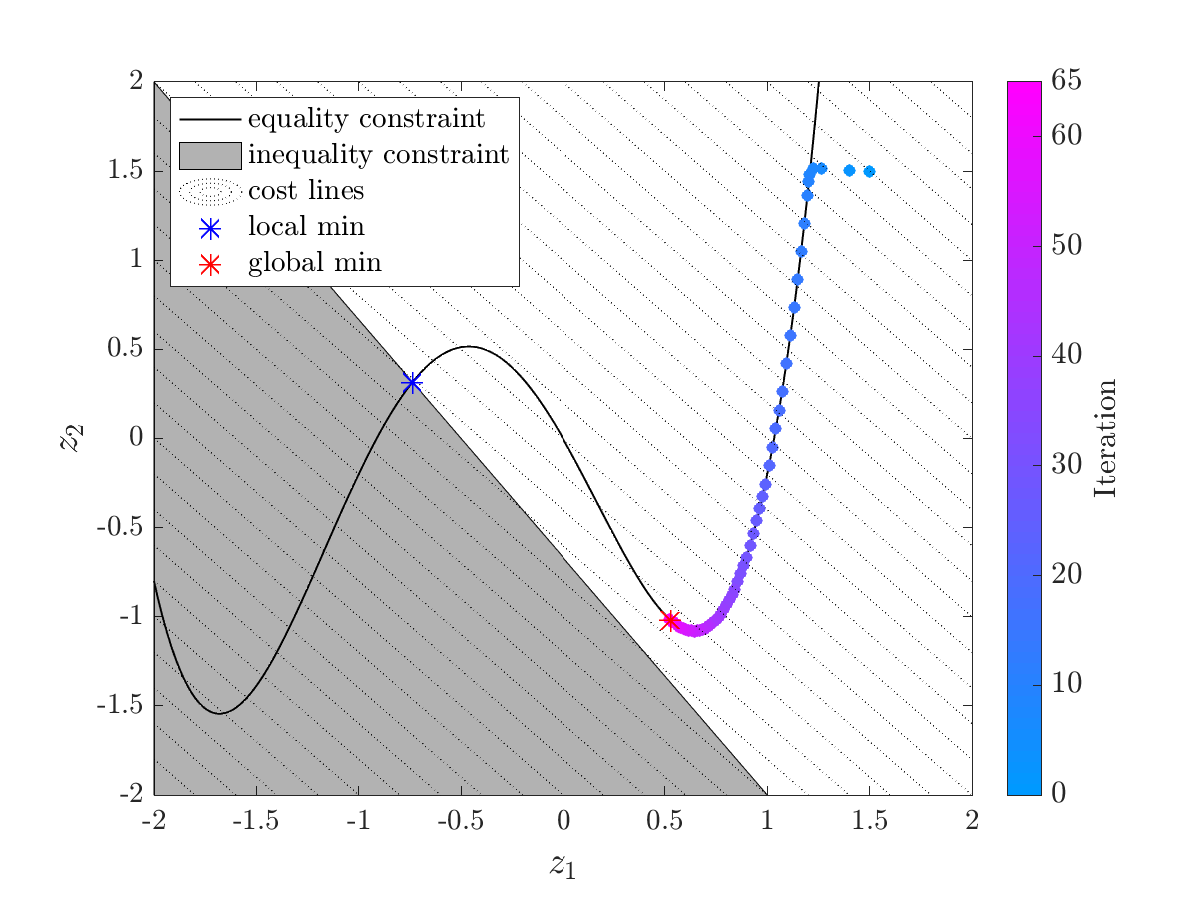
\includegraphics[width=0.33\textwidth]{figs/acc_toy_problem_relerr_cvrg_w2}} 
\subfloat[The performance metric $\pmet$ saturated to the $\left\lbrack0,1\right\rbrack$ interval solely for plotting. Color regions correspond to Figure~\ref{fig:scp_updates}.\label{fig:toy_prob_soln_c}]{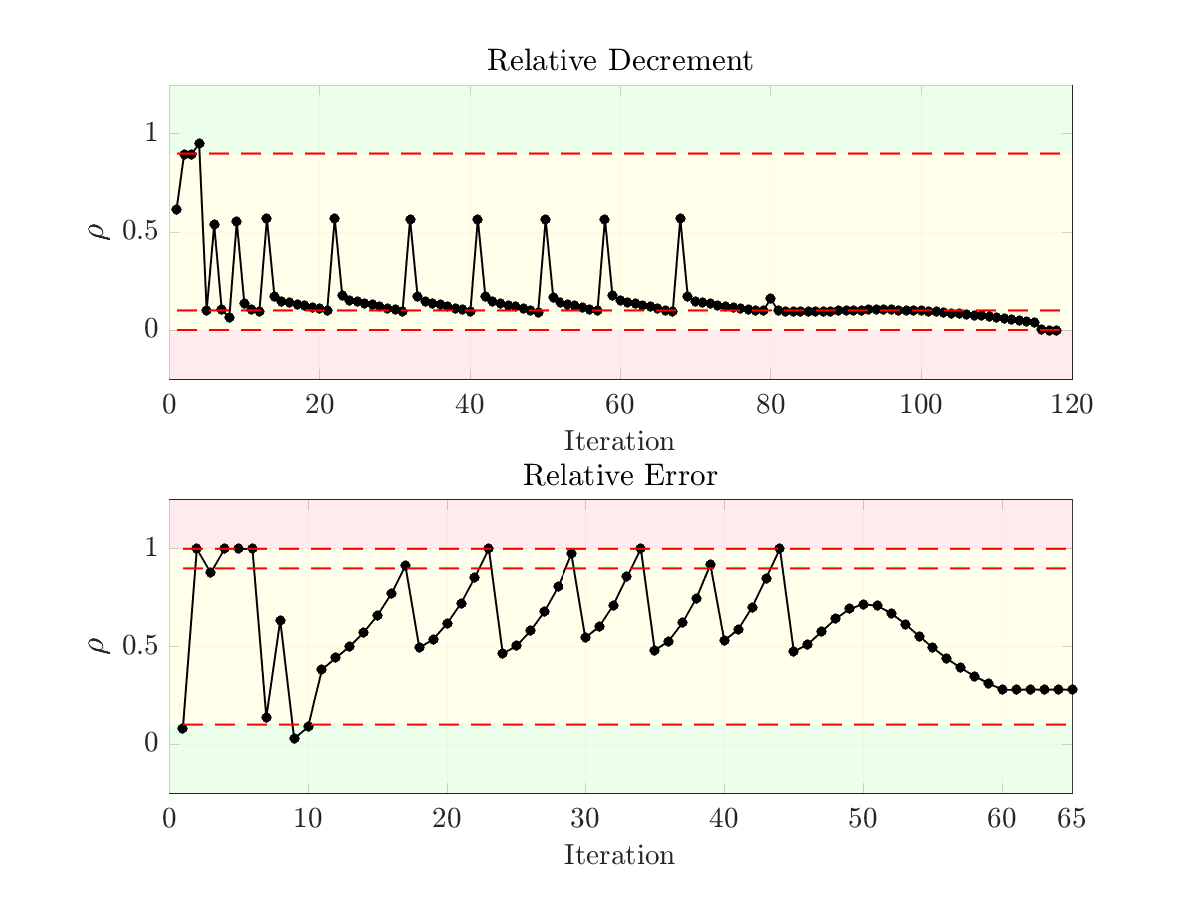
\includegraphics[width=0.33\textwidth]{figs/acc_toy_problem_rho_cvrg_w2}}
\caption{Solutions to Problem~\eqref{eq:toy_prob_cvx} showing the crawling phenomenon.}
\label{fig:toy_prob_soln}
\end{figure*}

% \subsubsection{Discussion}

It is important to recognize the nuances of this toy example correctly and resist the temptation to draw overly general conclusions from it. For other choices of initial condition, the crawling phenomenon is avoided. For example, convergence to the local minimum from an initial reference in the shaded gray region is quite rapid, often terminting in ten or fewer iterations. There are, however, relatively large regions in the upper-middle and upper-right of the area plotted in Figure~\ref{fig:toy_prob_soln} from which the phenomenon is observed. We are merely pointing out that the crawling phenomenon \textit{can} happen, not that it \textit{will}. 

It is obvious for this toy example that (i) the crawling phenomenon is occuring and (ii) that it occurs away from either minimum. This is only obvious because we know exactly where each minimum is (i.e., we can plot the cost lines and constraints). The trouble, in general, is that this is not possible. Higher dimensional non-convex problems for which no analytical solution is known may not permit the same observations that are obvious for this toy problem. Arriving at a local minimum indeed implies that adjacent iterates will be close together (in the sense that $\|\z^*-\zb\|$ is small), but what we have shown is that the converse is not necessarily true. The crawling phenomenon is perhaps observable\footnote{By observable, we mean that it can be determined if the algorithm is slowing down because it is close to an optimal solution or if it is exhibiting the crawling phenomenon.} by monitoring the value of $\rho$ for the behavior observed in Figure~\ref{fig:toy_prob_soln_c}. If this behavior is observed, then measures can be built into the algorithm to avoid it. 

%%%%%%%%%%%%%%%%%%%%%%%%%%%%%%%%%%%%%%%%%%%%%%%%%%%%%%%%%%%%%%%%%%%%%%%%%%%%%%%%

\section{POSSIBLE REMEDIES}\label{sec:remedies}

This section will discuss possible remedies to the crawling phenomenon that has been hitherto described. What can be discerned from Figure~\ref{fig:toy_prob_soln} is that SCP methods are typically quite good at quickly reaching feasibility. The cost of using virtual control dominates the original problems cost. Another advantage is the fact that rapid progress can be made towards an optimum in regions where the equality constraints are well-approximated by affine functions.

% \begin{itemize}
% \item discuss possible remedies; if we know we have a feasible start, what can we do?
% \item soft trust region methods?
% \end{itemize}

\section{CONCLUSIONS}\label{sec:conclusion}

As SCP algorithms become increasingly popular, it is important to recognize the limitations of such methods. At the same time, knowledge of the limitations provides an opportunity to design better algorithms that are not restricted in the same ways.


% \addtolength{\textheight}{-12cm}   % This command serves to balance the column lengths
                                  % on the last page of the document manually. It shortens
                                  % the textheight of the last page by a suitable amount.
                                  % This command does not take effect until the next page
                                  % so it should come on the page before the last. Make
                                  % sure that you do not shorten the textheight too much.

%%%%%%%%%%%%%%%%%%%%%%%%%%%%%%%%%%%%%%%%%%%%%%%%%%%%%%%%%%%%%%%%%%%%%%%%%%%%%%%%



%%%%%%%%%%%%%%%%%%%%%%%%%%%%%%%%%%%%%%%%%%%%%%%%%%%%%%%%%%%%%%%%%%%%%%%%%%%%%%%%



%%%%%%%%%%%%%%%%%%%%%%%%%%%%%%%%%%%%%%%%%%%%%%%%%%%%%%%%%%%%%%%%%%%%%%%%%%%%%%%%
% \section*{APPENDIX}

% Appendixes should appear before the acknowledgment.

% \section*{ACKNOWLEDGMENT}

% The preferred spelling of the word ÒacknowledgmentÓ in America is without an ÒeÓ after the ÒgÓ. Avoid the stilted expression, ÒOne of us (R. B. G.) thanks . . .Ó  Instead, try ÒR. B. G. thanksÓ. Put sponsor acknowledgments in the unnumbered footnote on the first page.



%%%%%%%%%%%%%%%%%%%%%%%%%%%%%%%%%%%%%%%%%%%%%%%%%%%%%%%%%%%%%%%%%%%%%%%%%%%%%%%%

\bibliographystyle{ieeetr}
\bibliography{references}


\end{document}
